\documentclass{article}
\usepackage{graphicx}
\usepackage{amsmath}
\usepackage[sorting=none]{biblatex}
\addbibresource{manual.bib}

\title{LIFTLINE Manual}
\author{Christopher C. Chinske}

\begin{document}
\maketitle
\newpage
\tableofcontents
\newpage
\section{Introduction}
\paragraph{}
LIFTLINE is a collection of MATLAB scripts and functions that
implement lifting-line theory.  It solves the monoplane equation to
estimate aerodynamic characteristics of a finite wing.  It also
provides capabilities to analyze shear force and bending moment along
the wing spar.
\subsection{Theory}
\paragraph{}
LIFTLINE implements lifting-line theory as described in \cite{bertin}
and \cite{anderson}.  The program estimates the spanwise circulation
of a finite wing.  Following from this result, the program can compute
the lift and vortex-induced drag coefficients.  The program can also
estimate structural characteristics, such as shear and bending moment
along the wing.
\paragraph{}
Classical lifting-line theory assumes incompressible flow, no wing
sweep, and linear airfoil section lift-curve slopes.  Currently,
LIFTLINE assumes:
\begin{enumerate}
\item Incompressible flow
\item No wing sweep (input required to properly draw planform)
\item Linear airfoil section lift-curve slopes
\item Symmetrical loading.
\end{enumerate}
Future versions of LIFTLINE will implement a modified lifting-line
theory and relax these assumptions.
\subsection{Program Organization}
\paragraph{}
The directory scripts\_aircraft contains input scripts that define
wing geometry and structural loads (e.g., fuel or stores).  The
directory scripts\_cases contains input scripts that define case
parameters.  These parameters may be overridden for certain analyses.
\subsection{Concept of Operations}
\paragraph{}
When analyzing a wing of finite span, the primary goals are to
determine: spanwise circulation, spanwise lift distribution, lift
coefficient, and vortex-induced drag coefficient.  Other goals might
include finding shear and bending moment for a cantilever wing,
determining rolling and yawing moments (for asymmetric loading), or
determining the stalling angle of attack.  The general procedure for
carrying out this analysis using LIFTLINE is outlined below.
\begin{enumerate}
\item Build an input script (aircraft) that defines the wing geometry.
\item Plot and verify the planform geometry.
\item Build an input script (case) that defines case parameters.
\item Run a grid convergence analysis, and update the case script.
\item For level flight, find the angle of attack for L = W, and update
  the case script.
\item Run case for a particular angle of attack to get spanwise
  circulation, spanwise lift distribution, lift coefficient, and
  vortex-induced drag coefficient.
\end{enumerate}
If desired, the lift and vortex-induced drag coefficients can be
computed across a range of angles of attack.  The spar shear and
bending moment can also be computed.
\paragraph{}
The function LIFTLINEUI provides an interactive user interface, which
aids the user in executing many of these tasks.
\paragraph{}
Advanced users can also call any of the program's library functions
directly.  In this way, users can build custom analysis routines.  The
figure below graphically depicts a typical workflow.
\newline
\newline
\fbox{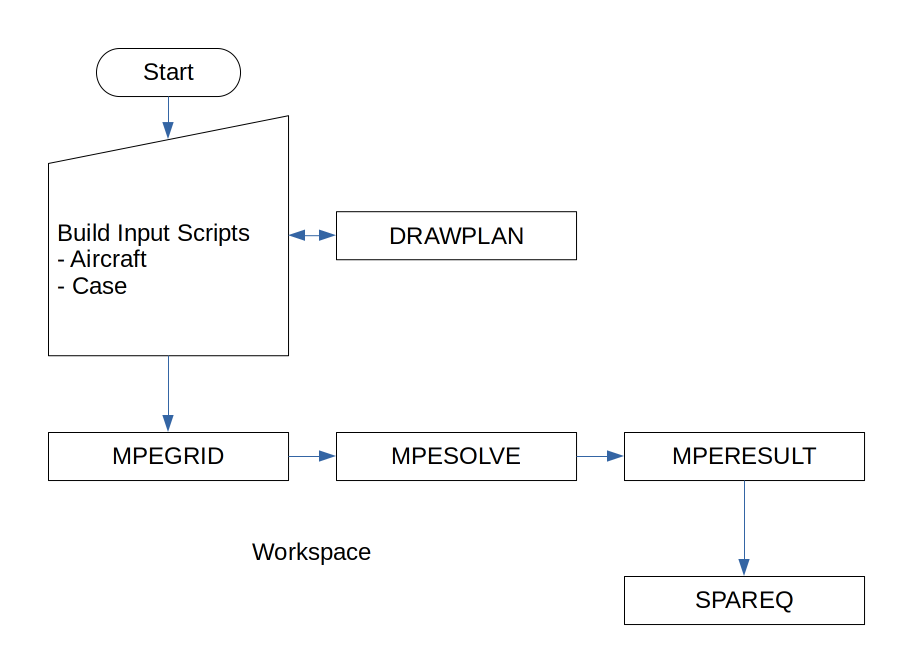
\includegraphics[width=\textwidth]{images/flowchart.png}}
\newline
\newline
\section{Definition of Inputs}\label{sec:doi}
\subsection{Planform Geometry}\label{sec:pg}
\fbox{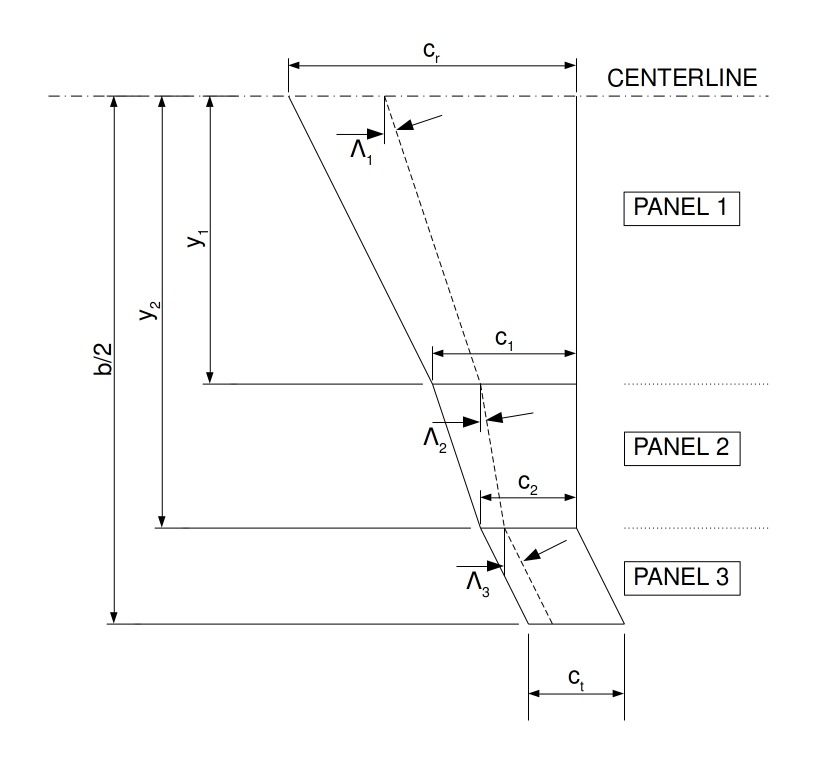
\includegraphics[width=\textwidth]{images/planform.png}}
\paragraph{}
An M-script in the folder scripts\_aircraft defines the wing geometry.
The required variables are given in the table below.  N panels compose
the semi-span.  For each row of clalp, alpzl, and clmax, the inboard
value applies immediately outboard of the panel's inboard
breakpoint.\\*\\*
\begin{tabular}{|l|l|p{2.5in}|c|}
  % --------------------------------------------------
  \hline
  \textbf{Variable Name} &
  \textbf{Dimension} &
  \textbf{Description} &
  \textbf{Units}
  \\
  \hline
  % --------------------------------------------------
%  var & dim &
%  description &
%  unit
%  \\
%  \hline
%  % --------------------------------------------------
  ybp & 1 x (N+1) &
  Spanwise coordinates of breakpoints [$0$, $y_1$, $y_2$, ..., $b/2$] &
  m
  \\
  \hline
  % --------------------------------------------------
  cbp & 1 x (N+1) &
  Chord at breakpoints [$c_r$, $c_1$, $c_2$, ..., $c_t$] &
  m
  \\
  \hline
  % --------------------------------------------------
  sweepa & 1 x N &
  Sweep angle (c/4) of each panel &
  deg
  \\
  \hline
  % --------------------------------------------------
  twista & 1 x N &
  Twist angle at tip of each panel &
  deg
  \\
  \hline
  % --------------------------------------------------
  clalp & N x 2 &
  Airfoil section lift-curve slope, $C_{l_\alpha}$.  Each row
  corresponds to a panel.  Column 1 is the inboard value.  Column 2 is
  the outboard value. &
  1/deg
  \\
  \hline
  % --------------------------------------------------
  alpzl & N x 2 &
  Airfoil section zero lift angle of attack, $\alpha_{0l}$.  Each row
  corresponds to a panel.  Column 1 is the inboard value.  Column 2 is
  the outboard value. &
  deg
  \\
  \hline
  % --------------------------------------------------
  clmax & N x 2 &
  Airfoil section maximum lift coefficient, $C_{l_{max}}$.  Each row
  corresponds to a panel.  Column 1 is the inboard value.  Column 2 is
  the outboard value. &
  -
  \\
  \hline
  % --------------------------------------------------
  b & Scalar &
  Span &
  m
  \\
  \hline
  % --------------------------------------------------
  S & Scalar &
  Reference wing area &
  m\^{}2
  \\
  \hline
  % --------------------------------------------------
  W & Scalar &
  Aircraft Weight &
  N
  \\
  \hline
  % --------------------------------------------------
\end{tabular}
\subsection{Structural Loads}\label{sec:sl}
\paragraph{}
An M-script in the folder scripts\_aircraft defines structural loads
(e.g., fuel or stores).  The function SPAREQ (Spar Equilibrium Shear
and Bending Moment) optionally uses the inputs ploads and uloads, as
defined below.\\*\\*
\begin{tabular}{|l|l|p{2.5in}|c|}
  % --------------------------------------------------
  \hline
  \textbf{Variable Name} &
  \textbf{Dimension} &
  \textbf{Description} &
  \textbf{Units}
  \\
  \hline
  % --------------------------------------------------
  ploads & R x 2 &
  Point loads applied along the wing.  Each row specifies a point
  load.  Column 1, y-values (meters).  Column 2, loads.  Negative
  loads values apply in the downward direction.  For example, a store
  would be input as a negative load.  Example:
  $\begin{bmatrix}1.2&-50\\2.1&-25\\\end{bmatrix}$ &
  N
  \\
  \hline
  % --------------------------------------------------
  uloads & R x 3 &
  Uniform distributed loads applied along the wing.  Column 1, inboard
  y-values (meters).  Column 2, outboard y-values (meters).  Column 3,
  load per unit span.  Negative loads values apply in the downward
  direction.  For example, a fuel tank would be input as a negative
  load.  Example:
  $\begin{bmatrix}1.1&2.2&-10\\2.0&4.0&-20\\\end{bmatrix}$ &
  N/m
  \\
  \hline
  % --------------------------------------------------
\end{tabular}
\subsection{Case Parameters}\label{sec:cp}
\paragraph{}
An M-script in the folder scripts\_cases defines case parameters
(i.e., run conditions).  Depending on the particular analysis, some of
these variables may be overridden or not required.\\*\\*
\begin{tabular}{|l|l|p{2.5in}|c|}
  % --------------------------------------------------
  \hline
  \textbf{Variable Name} &
  \textbf{Dimension} &
  \textbf{Description} &
  \textbf{Units}  
  \\
  \hline
  % --------------------------------------------------
  alpha\_r & Scalar &
  Angle of attack (root) &
  deg
  \\
  \hline
  % --------------------------------------------------
  ncoef & Scalar &
  Number of Fourier sine series coefficients &
  -
  \\
  \hline
  % --------------------------------------------------
  U & Scalar &
  Free-stream velocity &
  m/s
  \\
  \hline
  % --------------------------------------------------
  rho & Scalar &
  Density &
  kg/m\^{}3
  \\
  \hline
  % --------------------------------------------------
\end{tabular}
\section{Using LIFTLINEUI}
\paragraph{}
The function LIFTLINEUI provides an interactive user interface, which
aids the user in executing some of the program's functions.  This
section steps through a typical analysis scenario using the function
LIFTLINEUI.  This section assumes that you have installed the software
per the README and your MATLAB path is set to the top-level directory
of LIFTLINE.
\begin{enumerate}
  \item Build a script in the folder scripts\_aircraft that defines
    the planform geometry as described in section \ref{sec:pg}.  See
    the folder scripts\_aircraft for example M-files.
  \item Run the command
    \texttt{\textbf{drawplan(ybp,cbp,sweepa,twista)}}.  This plots the
    planform, and you can verify that the planform geometry looks
    correct.
  \item Build a script in the folder scripts\_cases that defines the
    case parameters as described in section \ref{sec:cp}.  See the
    folder scripts\_cases for example M-files.  Note, you can start
    with a small ncoef (for example, ncoef = 5) and a nominal angle of
    attack (for example, alpha\_r = 5).  Appropriate values will be
    determined as part of this analysis.
  \item Run the command \texttt{\textbf{liftlineui}}.
  \item Choose the option to ``Select aircraft script,'' and select
    the input script that defines the planform geometry.
  \item Choose the option to ``Select run conditions script,'' and
    select the input script that defines the case parameters.
  \item Choose the option to ``Continue.''
  \item Choose the option to execute a ``Grid Convergence Analysis.''
  \item Enter the desired accuracy (significant figures) for the lift
    coefficient.
  \item Enter the desired accuracy (significant figures) for the
    vortex-induced drag coefficient.
  \item The program will output the required ncoef to achieve the
    desired accuracy.  Update the case parameters script with this
    value for ncoef.
  \item Rerun \texttt{\textbf{liftlineui}} using the same procedure,
    but this time, choose the option to ``Find AoA for L = W.''
  \item The program will output the required alpha\_r for level
    flight.  Update the case parameters script with this value for
    alpha\_r.
  \item Rerun \texttt{\textbf{liftlineui}} using the same procedure.
    Choose the option to ``Run Case as Defined in Run Conditions
    Script.''  This will output the wing lift coefficient and wing
    vortex-induced drag coefficient for the particular case.  This
    will also plot the spanwise circulation and spanwise section lift
    coefficient.
  \item Rerun \texttt{\textbf{liftlineui}} using the same procedure.
    Choose the option for ``AoA Range.''  This will plot the wing lift
    coefficient and wing drag polar over a range of angles of attack.
  \item Rerun \texttt{\textbf{liftlineui}} using the same procedure.
    Choose the option for ``Spar Shear and Bending Moment.''  This
    will plot the spanwise shear and bending moment
    diagrams.\footnote{Currently, this option in LIFTLINEUI only
      considers the aerodynamic wing loading and does not use a
      structural loads script as described in section \ref{sec:sl}.
      To include structural loads, the user must call the function
      SPAREQ directly.}
\end{enumerate}
Some choices will save output variables in a timestamped MAT file in the
current folder.
\section{Function Reference}
\subsection{Symmetric Solvers}
\paragraph{}
The symmetric solvers (i.e., symmetrical wing loading) use
inputs/outputs as defined below.  N is the number of Fourier sine
series coefficients.\\*\\*
\begin{tabular}{|l|l|p{2.5in}|c|}
  % --------------------------------------------------
  \hline
  \textbf{Variable Name} &
  \textbf{Dimension} &
  \textbf{Description} &
  \textbf{Units}
  \\
  \hline
  % --------------------------------------------------
  alpha\_r & Scalar &
  Angle of attack (root) &
  deg
  \\
  \hline
  % --------------------------------------------------
  ncoef & Scalar &
  Number of Fourier sine series coefficients &
  -
  \\
  \hline
  % --------------------------------------------------
  theta & 1 x N &
  Transformed spanwise coordinate &
  rad
  \\
  \hline
  % --------------------------------------------------
  y & 1 x N &
  Spanwise coordinate &
  m
  \\
  \hline
  % --------------------------------------------------
  c & 1 x N &
  Chord &
  m
  \\
  \hline
  % --------------------------------------------------
  a0 & 1 x N &
  Section lift-curve slope &
  1/rad
  \\
  \hline
  % --------------------------------------------------
  alpha & 1 x N &
  Section angle of attack &
  rad
  \\
  \hline
  % --------------------------------------------------
  alpha\_zl & 1 x N &
  Section zero lift angle of attack &
  rad
  \\
  \hline
  % --------------------------------------------------
  clmax\_vec & 1 x N &
  Section maximum lift coefficient &
  -
  \\
  \hline
  % --------------------------------------------------
  An & 1 x N &
  Fourier coefficients [$A_1$, $A_3$, ..., $A_{2N-1}$] &
  -
  \\
  \hline
  % --------------------------------------------------
  U & Scalar &
  Free-stream velocity &
  m/s
  \\
  \hline
  % --------------------------------------------------
  Gamma & 1 x N &
  Circulation &
  m\^{}2/s
  \\
  \hline
  % --------------------------------------------------
  CL & Scalar &
  Wing lift coefficient &
  -
  \\
  \hline
  % --------------------------------------------------
  CDv & Scalar &
  Wing vortex-induced drag coefficient &
  -
  \\
  \hline
  % --------------------------------------------------
  cl & 1 x N &
  Section lift coefficient &
  -
  \\
  \hline
  % --------------------------------------------------
  V & 1 X N &
  Shear &
  N
  \\
  \hline
  % --------------------------------------------------
  M & 1 X N &
  Bending Moment &
  N*m
  \\
  \hline
  % --------------------------------------------------
  M\_root & 1 X N &
  Root Bending Moment &
  N*m
  \\
  \hline
  % --------------------------------------------------  
\end{tabular}
\begin{description}
  \item[mpegrid] Returns vectors of coordinates and section values at
    N spanwise locations from $0 \leq y \leq b/2$.
  \item[$>>$] [theta,y,c,a0,alpha,alpha\_zl,clmax\_vec] = \ldots\\*
    mpegrid(ybp,cbp,twista,clalp,alpzl,clmax,alpha\_r,ncoef)
  \item[mpesolve] Solves the monoplane equation for symmetrical
    loading.
  \item[$>>$] An = mpesolve(theta,c,a0,alpha,alpha\_zl,b)
  \item[mperesult] Returns aerodynamic results based on the
    output of MPESOLVE.
  \item[$>>$] [Gamma,CL,CDv,cl] = mperesult(An,theta,c,U,b,S)
  \item[spareq] Returns shear and bending moment for the cantilever
    wing.  Optional input arguments ploads and uloads specify point
    loads and uniform distributed loads along the wing, respectively.
    See section \ref{sec:sl} for more information on defining
    structural loads.
  \item[$>>$] [V,M,M\_root] = spareq(Gamma,y,rho,U)
  \item[$>>$] [V,M,M\_root] = spareq(Gamma,y,rho,U,ploads,uloads)
\end{description}
\subsection{Plotting}
\paragraph{}
Use the MATLAB help command to display usage instructions for the
plotting functions (e.g., \texttt{\textbf{help mpeplot}} for help
using the MPEPLOT function).
\begin{description}
\item[drawplan] Plots the planform.
\item[mpeplot] Utility function to plot results.
\end{description}
\newpage
\printbibliography
\end{document}
